\documentclass[a4]{report}
\usepackage[T1]{fontenc}
\usepackage[applemac]{inputenc}
\usepackage[danish]{babel}
\usepackage{amsmath,amssymb,amsthm} % matematik
\usepackage{booktabs} % p�nere tabeller
\usepackage[pdftex]{graphicx}
\usepackage{fancyhdr} % hoved- og sidefod
\pagestyle{fancy} 

\begin{document}
\chapter{Mit f�rste \LaTeX dokument!}
\subsection {Abstract}
In this project it is our task to implement a circuit on the FPGA board, that can display a square patterns in the seven-segment LED display. This pattern must be able to  circulated the display both clockwise and counterclockwise.

\begin{figure}[!htbp] 
	\centering 
		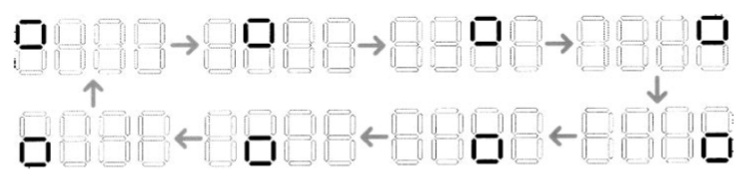
\includegraphics[scale=0.4]{fig/DigitBox.jpg} 
	\caption{Moving square on 7-segment display}
	\label{fig:1} 
\end{figure}

The circuit will switch directions dependently to the position of Switch1and Button1 will act as reset for the system. Furthermore a clock should be implemented with a slow running clock generator to display the "Moving square box".


\end{document}
